\subsection{Условный экстремум функции многих переменных}
\begin{tbox}{Условный экстремум}
	Экстремум функции, на аргументы которой наложены дополнительные условия связи, называется \textbf{условным экстремумом}.
\end{tbox}

\begin{figure}[h]
	\centering
	\begin{minipage}[c]{0.4\linewidth} % [c] для выравнивания по центру
		\centering
		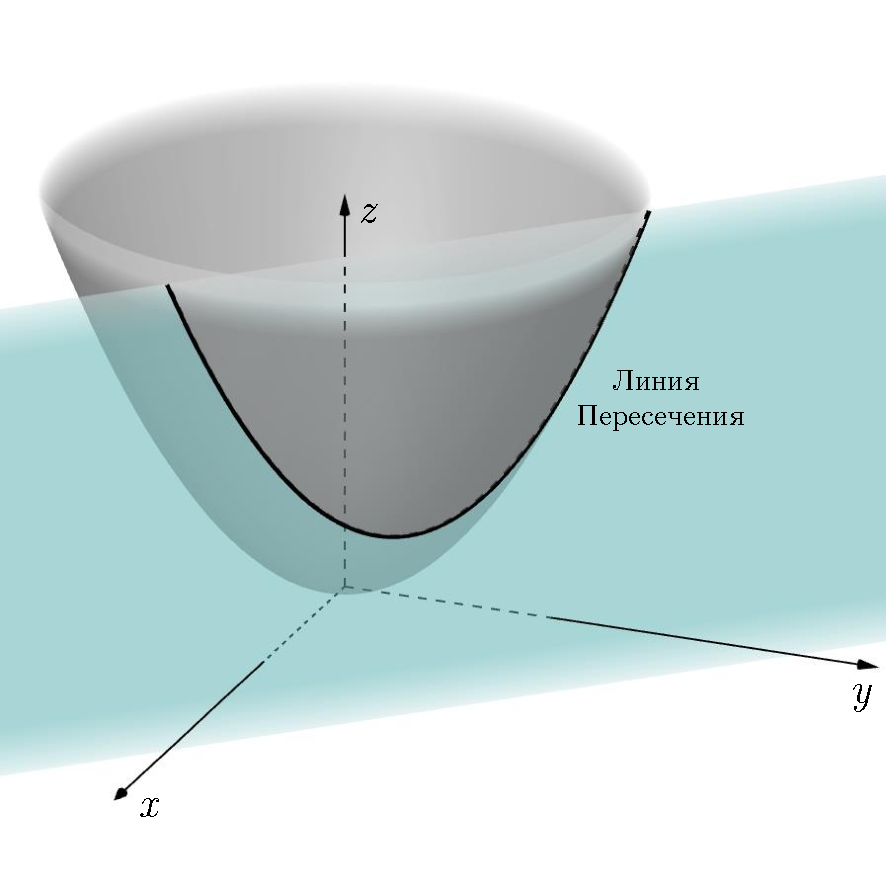
\includegraphics[width=\linewidth]{7.pdf} % Укажите высоту, если нужно
		\caption{Графическая иллюстрация условного экстремума}
		\label{fig:17}
	\end{minipage}
\end{figure}

\subsubsection*{Пример условного экстремума (Рис. \ref{fig:17})}
Пусть $z = x^2 + y^2$ при условии связи $x + y = 1$. Точка $M_0(0, 0)$ является точкой минимума (абсолютный экстремум).

Экстремум на линии пересечения плоскости $x + y = 1$ и параболоида $z = x^2 + y^2$ является условным экстремумом. Для его нахождения выразим переменную $y$ из условия связи и подставим в уравнение функции.

Получаем функцию одной независимой переменной, которую исследуем на экстремум:
\begin{gather*}
	x + y = 1 \Rightarrow y = 1 - x, \\
	z = x^2 + y^2 = x^2 + (1 - x)^2 = x^2 + 1 - 2x + x^2 = 2x^2 - 2x + 1.
\end{gather*}
\begin{align*}
	z_x' &= 4x - 2 = 0 \Rightarrow x = \frac{1}{2} \text{ — стационарная точка}, \\
	z_{xx}'' &= 4 > 0 \Rightarrow x = \frac{1}{2} \text{ — точка минимума функции } z = 2x^2 - 2x + 1, \\
	y &= 1 - x = 1 - \frac{1}{2} = \frac{1}{2}; \quad \left(\frac{1}{2}; \frac{1}{2}\right) \text{ — точка условного минимума}, \\
	z_{\text{min}} &= z\left(\frac{1}{2}; \frac{1}{2}\right) = \left(\frac{1}{2}\right)^2 + \left(\frac{1}{2}\right)^2 = \frac{1}{2}.
\end{align*}

Если уравнений связи несколько или они нелинейные, то свести задачу условного экстремума к исследованию функций одной или нескольких переменных бывает сложно. В этом случае применяют \textit{метод неопределённых множителей Лагранжа}.

\begin{tbox}{Метод множителей Лагранжа}
	В общем случае задача ставится следующим образом:

	Пусть задана функция $y = f(x_1, x_2, \dots, x_k)$, а независимые переменные $x_1, x_2, \dots, x_k$ связаны условиями, число которых меньше числа независимых переменных:
	\begin{equation} \label{eq:8.1}
		\begin{cases}
			\varphi_1(x_1, x_2, \dots, x_k) = 0, \\
			\varphi_2(x_1, x_2, \dots, x_k) = 0, \\
			\dots, \\
			\varphi_n(x_1, x_2, \dots, x_k) = 0,
		\end{cases}
		\quad n < k.
	\end{equation}

	Составим функцию Лагранжа:
	\begin{multline} \label{eq:8.2}
		L = f(x_1, x_2, \dots, x_k) + \lambda_1 \varphi_1(x_1, x_2, \dots, x_k) + \lambda_2 \varphi_2(x_1, x_2, \dots, x_k) + \dots \\ \dots + \lambda_n \varphi_n(x_1, x_2, \dots, x_k).
	\end{multline}

	Здесь $\lambda_1, \lambda_2, \dots, \lambda_n$ — неопределённые множители Лагранжа, которые находятся из условий:
	\begin{equation*}
		\begin{cases}
			\frac{\partial L}{\partial \lambda_1} = \varphi_1(x_1, x_2, \dots, x_k) = 0, \\
			\frac{\partial L}{\partial \lambda_2} = \varphi_2(x_1, x_2, \dots, x_k) = 0, \\
			\dots, \\
			\frac{\partial L}{\partial \lambda_n} = \varphi_n(x_1, x_2, \dots, x_k) = 0.
		\end{cases}
	\end{equation*}

	Задача поиска условного экстремума сводится к поиску обычного экстремума для функции Лагранжа \eqref{eq:8.2}. Необходимое условие экстремума:
	\begin{equation} \label{eq:8.3}
		\begin{cases}
			\frac{\partial L}{\partial x_1} = 0, \\
			\frac{\partial L}{\partial x_2} = 0, \\
			\dots, \\
			\frac{\partial L}{\partial x_k} = 0, \\
			\frac{\partial L}{\partial \lambda_1} = \varphi_1(x_1, x_2, \dots, x_k) = 0, \\
			\frac{\partial L}{\partial \lambda_2} = \varphi_2(x_1, x_2, \dots, x_k) = 0, \\
			\dots, \\
			\frac{\partial L}{\partial \lambda_n} = \varphi_n(x_1, x_2, \dots, x_k) = 0.
		\end{cases}
	\end{equation}

	Получаем систему $k + n$ уравнений относительно неизвестных $x_1, x_2, \dots, x_k$ и $\lambda_1, \lambda_2, \dots, \lambda_n$.

	Решая систему \eqref{eq:8.3}, находим стационарные точки $M_0(x_{0_1}, x_{0_2}, \dots, x_{0_k})$ и значения множителей Лагранжа $\lambda_1 = \lambda_{0_1}, \lambda_2 = \lambda_{0_2}, \dots, \lambda_n = \lambda_{0_n}$.
\end{tbox}

\begin{tbox}{Второй дифференциал функции Лагранжа}
	Дальнейшее исследование стационарных точек на экстремум связано с анализом знака второго дифференциала с учётом дифференциальных условий связи.

	Второй дифференциал функции Лагранжа в точке $M_0$:
	\begin{equation*}
		\begin{aligned}
			d^2 L(M_0) = &\frac{\partial^2 L(M_0)}{\partial x_1^2} dx_1^2 + \frac{\partial^2 L(M_0)}{\partial x_2^2} dx_2^2 + \dots + \frac{\partial^2 L(M_0)}{\partial x_k^2} dx_k^2 \, + \\
			&+ 2 \frac{\partial^2 L(M_0)}{\partial x_1 \partial x_2} dx_1 dx_2 + 2 \frac{\partial^2 L(M_0)}{\partial x_1 \partial x_3} dx_1 dx_3 + \dots + 2 \frac{\partial^2 L(M_0)}{\partial x_{k-1} \partial x_k} dx_{k-1} dx_k.
		\end{aligned}
	\end{equation*}

	Так как переменные $x_1, x_2, \dots, x_k$ связаны условиями \eqref{eq:8.1}, их дифференциалы также связаны. Найдём дифференциалы условий связи в точке $M_0$:
	\begin{gather*}
		\varphi_1(x_1, x_2, \dots, x_k) = 0 \quad \Big| \, d, \\
		d\varphi_1(M_0) = \frac{\partial \varphi_1(M_0)}{\partial x_1} dx_1 + \frac{\partial \varphi_1(M_0)}{\partial x_2} dx_2 + \dots + \frac{\partial \varphi_1(M_0)}{\partial x_k} dx_k = \sum_{i=1}^k \frac{\partial \varphi_1(M_0)}{\partial x_i} dx_i = 0, \\
		\varphi_2(x_1, x_2, \dots, x_k) = 0 \quad \Big| \, d, \\
		d\varphi_2(M_0) = \frac{\partial \varphi_2(M_0)}{\partial x_1} dx_1 + \frac{\partial \varphi_2(M_0)}{\partial x_2} dx_2 + \dots + \frac{\partial \varphi_2(M_0)}{\partial x_k} dx_k = \sum_{i=1}^k \frac{\partial \varphi_2(M_0)}{\partial x_i} dx_i = 0, \\
		\dots, \\
		\varphi_n(x_1, x_2, \dots, x_k) = 0 \quad \Big| \, d, \\
		d\varphi_n(M_0) = \frac{\partial \varphi_n(M_0)}{\partial x_1} dx_1 + \frac{\partial \varphi_n(M_0)}{\partial x_2} dx_2 + \dots + \frac{\partial \varphi_n(M_0)}{\partial x_k} dx_k = \sum_{i=1}^k \frac{\partial \varphi_n(M_0)}{\partial x_i} dx_i = 0.
	\end{gather*}

	Исследуем знак второго дифференциала с учётом этих условий.
\end{tbox}

\subsubsection*{Пример метода множителей Лагранжа}
Задана функция $z = x^2 + xy + y^2$ с условием $x + y = 2$, где $x$ и $y$ — независимые переменные. Введём функцию Лагранжа:
\[
L = x^2 + xy + y^2 + \lambda(x + y - 2).
\]

Частные производные:
\[
\begin{cases}
	2x + y + \lambda = 0, \\
	x + 2y + \lambda = 0, \\
	x + y = 2.
\end{cases}
\]

Решаем систему:
\[
y = 2 - x, \quad 2x + (2 - x) + \lambda = 0, \quad x + 2(2 - x) + \lambda = 0.
\]
\[
x = 1, \quad y = 1, \quad \lambda = -3.
\]

Вторые производные:
\[
\frac{\partial^2 L}{\partial x^2} = 2, \quad \frac{\partial^2 L}{\partial x \partial y} = 1, \quad \frac{\partial^2 L}{\partial y^2} = 2.
\]

Квадратичная форма:
\[
d^2 L = 2 dx^2 + 2 dx dy + 2 dy^2.
\]
При $dx + dy = 0$ (так как $x + y = 2$):
\[
d^2 L = 2 dx^2 > 0.
\]

Точка $(1, 1)$ — условный минимум. Значение:
\[
z(1, 1) = 3.
\]

\textbf{Ответ:} $z_{\text{min}} = 3$ в точке $(1, 1)$.